\chapter{Theoretical Framework}
% Explain concepts that we rely upon throughout the report. 

%This chapter will introduce the theoretical framework of the project.

The following sections will include an explanation of the underlying theory and physics of racing, an introduction to the challenges of digital simulation and an overview of and motivation for machine learning concepts used in the project. 

\section{Racing Theory}
\label{racing_theory}
% Started to re-write, maybe usable
% Understanding racing theory is crucial to understand what the goal of the AI driver behaviour is, and to discuss what the requirements for it are. Racing theory involves both good practises and the reasons behind them. 
% As mentioned, the type of competition is a single car performing a time attack. The goal is to drive around a track with as little time as possible. It is a little harder to 

As mentioned in \ref{purpose}, the goal of the project is to create a racing AI able to drive a car around a racing track as quickly as possible. Racing tracks are normally broad enough to allow many different paths for the driver. Different paths may differ in length but also affect the possible speed. Time is the result from both distance and speed according to the following formula: \(t = \frac{d}{v}\), where $d$ is the distance driven and $v$ is the average speed. The process of minimising the time is a process of both minimising the distance driven and maximising the speed. 

%\begin{equation}
%t = \frac{d}{v}
%\end{equation}


The next subsection will briefly describe the physics of racing. It is a core part of understanding how professional drivers drive, as will be described in the second next subsection.

\subsection{Underlying Physics of Racing}
%%Baka in källor, bl.a. Edmond
A moving car has momentum. In order to change the momentum, for example to accelerate, decelerate, or change the direction of movement, a force must be applied. These forces are applied through the tyres. This is a restricting factor for cars since the available traction, which is the amount of force that can be applied through the tyres, is limited. If the applied force exceeds the available traction, the tyres will slide or spin \cite{beckman}. 

The brakes are generally very efficient and are mostly limited by the traction of the tyres, whereas accelerating is limited by the torque of the engine. Additionally, a car travelling forward is slowed by the air drag. When the car brakes, the tyres and the drag will work together, but an accelerating car has to work against the drag. These aspects make cars accelerate slower than they can decelerate.

As described by Newtonian mechanics, the kinetic energy of a moving object increases quadratically with the speed. A consequence of higher speed is that a greater force is required to change the momentum. The acceleration required to make a moving object stay in a circular motion is \(a_c=\frac{v^2}{r}\)  \cite{beckman}. Using \(F=ma\), the formula is transformed to: 
%Accelerating and braking takes longer time and the turning radius is larger. The The turning radius for a circular motion is:

\begin{equation}
\label{equation:turn_radius}
a_c = \frac{v^2}{r} 
\rightarrow
\frac{F_c}{m} = \frac{v^2}{r} 
\rightarrow
r = \frac{mv^2}{F_c}
\end{equation}

\noindent
Where $a_c$ is the central acceleration, $v$ is the speed, $r$ is the radius of the circular motion, $F_c$ is the central force and $m$ is the mass of the car. 

The car cannot turn as much when it accelerates or brakes. When a car accelerates or brake, the weight of the car transfer slightly and the amount of pressure on the tyres will change, changing the traction capabilities. This limits the amount a car accelerates or brake and turn at the same time \cite{beckman}. The effect is further increased since both turning and changing the speed requires traction and share the same traction budget. Thus turning the car uses some of the available traction which reduces the amount the car can accelerate \cite{beckman, edmondson}. 

% Turning changing velocity requires traction, thus 
%The effect is further increased as the tyres cannot produce traction for multiple directions as well as for a single direction \cite{beckman}. 

Due to the shape of a racing car, air drag contribute to the traction by pushing the car down. This effect, which is called down force, grows as the speed increases \cite{beckman}.

\subsection{Introduction to Racing Lines}
\label{racing_theory:lines}
A racing line denotes the path a car drive around the track. It is an expression that include both the positioning and speed of the car.

% OLD version
%As previously mentioned, driving fast and driving short are the key aspects to optimise, but they sometimes opposite each other. If the car drives fast, the turning radius is increased and the car might need to drive a longer path, which may take longer time in total. 

%However, if the car exits a corner with a higher speed, it can benefit from a reduced time spent in the next section. It is therefore generally beneficial to prioritise higher speed on longer sections \cite{beckman}, as the difference in speed will accumulate more time.

%A typical behaviour is therefore to position the car on the opposite side of where a corner is turning. This enables a larger turning radius. The car brakes as late as possible to not loose time on the previous section, but turns most intensively rather early in the corner, so that it can start accelerating for the next section as early as possible. This corner will result in a late apex.

As mentioned in \ref{racing_theory}, driving fast and driving short are the key aspects to optimise in order to minimise lap times, but they sometimes counteract each other. If the car drives fast, the turning radius is increased and the car might need to drive a longer path, which may take longer time in total \cite{edmondson}. 

It is generally good to keep as high speed as possible and to drive close to the inner corners. The position where the racing line is closest to the inner corner is called the apex. Depending on the situation the driver may take an early, middle, or late apex, as conceptually illustrated in figure \ref{figure:apex_variants}.

\begin{figure}[H]
    \centering
    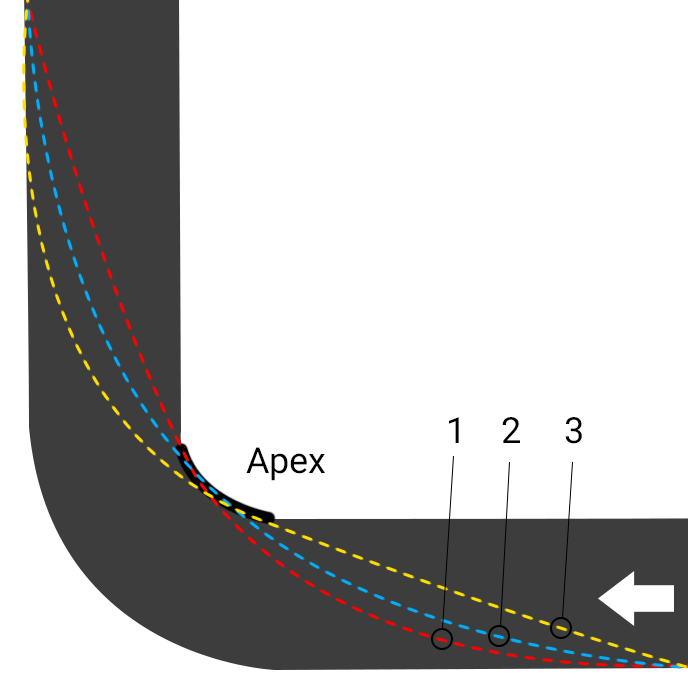
\includegraphics[width=0.5\textwidth]{race_lines}
    \caption{The point where the racing line hit the inner corner is called apex. Line 1 has a late apex point, line 2 a mid apex point and line 3 an early apex point as the corner is taken from the right direction.}
    \label{figure:apex_variants}
\end{figure}

\noindent
A driver usually need to brake before a corner in order to keep the turning radius down and not crash into the corner. But, even at a suitable speed, the race line seldom in the shape of a circle sector. Competitive drivers do to some degree accelerate or brake at the same time as turning \cite{edmondson}. The traction budget is a limiting factor, bu, if handled correctly, it can be used to increase speed and reduce distance driven. 

If the car exits a corner with a higher speed, it can benefit from a reduced time spent in the next section. It is therefore generally beneficial to prioritise higher speed on longer sections \cite{beckman, edmondson}, as the difference in speed will accumulate to a larger time difference. The optimal behaviour is therefore to break early so that a large portion of the turning can be done early in the corner, and then start to accelerate early, resulting in a late apex. This type of corner is often referred to as a type 1 corner \cite{edmondson}.

However, when a corner ends a straight section and is not followed by another straight, it is normally best to brake and steer late to benefit most of the high speed before the corner \cite{edmondson}. This line will hit an early apex and it is often referred to as a type 2 corner.

The last type is the type 3 corner, which is any corner that do not fall into the type 1 or type 2 categories \cite{edmondson}. These corners are not adjacent to any straight section long enough for any of the two first racing lines to be beneficial. The appearance of the optimal racing line may vary drastically depending on the situation and the performance of the car.

\subsection{Requirements on the simulator}
\label{requirements}
The purpose of this study is to evaluate how well a machine learning algorithm can learn the key aspects of an effective racing behaviour. Some of the aspects that will be evaluated are conceptual positioning throughout corners, timing and speed management.

If the behaviour of the AI is to be assessed in comparison to real world racing theory, the optimal behaviour in the simulated environment must be similar to the optimal behaviour in reality. The simulation may approximate certain aspects or neglect details, as long as the general characteristics remain, and the best practises in racing theory are still optimal. 

Type 1 and 2 corners have typical racing lines that conceptually do not depend on miniature differences in performance, although the exact positioning and timing do. In contrast, the optimal racing line for type 3 corners vary largely depending on the situation and performance of the car. The behaviour in those corners might be interesting to analyse, but not in the purpose of comparing to the generic best practises.

Some fundamental aspects for the simulator is the turning radius and the relationship between acceleration and retardation. The turning radius forces the driver to control the speed appropriately and find a balance between the length of racing lines and speed. It requires the driver to position the car well and to plan ahead. Acceleration need be slow enough for an increase of exit speed in type 1 corners to outperform a slightly shorter path, and also than accelerating, so that the speed prioritisation is correct for the type 1 and type 2 corners. 

Weight transfer and the traction budget are important aspects to consider when for a driver that drives to the limits of the cars performance. Not considering it in the simulation, would likely make the optimal timing for the different stages blend together slightly. It does, however, not change the general racing lines for type 1 and type 2 corners as it only changes timing and positioning slightly. Aspects such as tyre wear and temperature changes the performance of the car and how much the driver want to push the limits, but do not have a considerable change to the local behaviour. 

In summary, the key aspects to consider in the physics simulation is the turning radius and that the car accelerates slower than it brakes. Aspects such as weight transfer and the complexity the traction budget model would increase how well the simulator resemble reality, but not change the generic behaviour for the type 1 and 2 corners. 

\section{Digital Simulation}
% - Discrete steps
% - Numerical errors

% Should we keep this section or integrate it into the implementation of the simulator section?? 

Computers have been utilised throughout the project to simulate the physics of a racing car. However, digital simulation introduces errors that potentially could affect the result. This section will present some of the key aspects of digital simulation. 

A digital computer cannot due to its discrete nature store or calculate real numbers exactly. Instead something called floating point numbers are used. Floating point numbers is a way to represent real numbers as discrete values. It works by storing the significant digits of a number together with a value representing an exponent. The floating point number can be calculated by multiplying the significant digits with a fixed base raised to the stored exponent.

The simulator holds a state of what it simulates. The simulation progress by calculating what the new state should be after an amount of time have elapsed. One of the limitations of this way of simulating is that it difficult to take in to account events that should have occurred during the time slice, or multiple degrees of derivatives. 

Due to computers being unable to handle continuous calculations they must rely on models of reality. This will introduce numerical errors in the calculations. It is therefore important to motivate that the errors introduced are small enough for it to not decrease the quality of the simulation.



\section{Machine Learning}
Machine learning is the field of study that concentrates on algorithms that can be said to learn \cite{glossary}. This section will cover the machine learning theory and concepts that were considered and used within the project. Furthermore, the suitability of the different algorithms within the problem domain will be discussed.  

\subsection{Artificial Neural Networks as Knowledge Model}
Machine learning algorithms require some representation of knowledge. One such knowledge model that is in wide use is the Artificial neural network (ANN). An ANN is a mathematical model that mimics the structure of the human brain. 

The human brain is a large network of nerve cells called neurons. The neuron is a cell capable of firing an electrical pulse that can be transmitted electrically or chemically to other neurons via connections called synapses. A neuron fires its pulse when the accumulated incoming signals from other neurons reach a certain threshold. Akin to a biological neural network, an ANN is a network of artificial neurons or nodes. Each node has an output value which is calculated from a set of incoming connections. The connections are a set of weighted edges. The edges are directed, which means that they represent a signal flow from one neuron to another in the direction of the edge.

An ANN can represent a mathematical function by connecting a set of input nodes to a set of output nodes, thus representing a mapping from the input space to the output space. Between the input and output nodes, additional nodes called hidden nodes may exist. Output nodes and hidden nodes may not only be connected to the input nodes, but also other hidden nodes. These connections is what constitutes the neural networks. 

The function is calculated by setting the values of the input nodes and then propagating the values through the network. The propagation of values works by feeding the value of one node to the others via a nodes outbound edges. The value of a node $v$ is calculated by passing the weighted sum of the values on the incoming connections to an activation function $\phi(x)$. The full formula is shown in equation \ref{eq:neuron} where $w_i$ is the weight and $v_i$ is the value of an incoming connection 

\begin{equation}
    v = \phi (\sum_i{[w_i v_i]} + b)
    \label{eq:neuron}
\end{equation}


\noindent

The choice of activation function is arbitrary but will greatly affect the nature of the represented function. Usually a sigmoid-function is used, which is a smooth step function on the form:

\begin{equation}
    S(t) = L + \frac{a}{1 + e^{-bt}}
\end{equation}

\noindent
Here $L$ denotes the lower bound of the function, $a$ defines the range of values and $b$ defines the steepness of the function. The value-range of the function is $[L, L+a]$. 

An ANN with at least two layers of hidden neurons and a sigmoid function as its activation function can be used to approximate any real function, furthermore the accuracy increases with the number of neurons \cite{mitchel:approximation}. The function approximated by an ANN can be changed by changing the topology or weights of the network. Artificial neural networks are thus useful for fitting curves to data. 



\subsection{Supervised Learning}
Supervised learning is the process of learning with a teacher or learning from examples \cite{haykin:supervised}. A large set of example data consisting of pairs of input configurations and the corresponding correct output is used. The learning process works by letting the knowledge model, for example a neural network, predict the correct output for given inputs in the data set. The knowledge model is then corrected in order to better predict the correct output. Algorithms that learn by induction often fall into the supervised learning category \cite{glossary}. 

Supervised learning algorithms are useful when the goal is to create an accurate prediction model from a large set of example data. As mentioned in chapter \ref{introduction}, it is used as a key compartment for autonomous vehicles \cite{?}. This is a good indication that it is possible to use for complex control tasks.

However, the primary goal of this project is to create an AI not by defining how it should behave but by defining what it should strive for. Supervised learning could certainly be used to create a racing AI that for example emulates a professional driver. It could also be used to solve one part of the problem, for example learning where to position the car on the track. However, the scarcity of available data limits the use of these algorithms.  



\subsection{Unsupervised Learning}
Unsupervised learning is a type of machine learning that in contrast to supervised learning does not learn to predict or approximate a correct output given an input, but rather learn to group sets of inputs into categories based on the input values. These algorithms are prevalent in data mining and other areas where clustering is useful. 



\subsection{Reinforcement Learning}
\label{theory:reinforcement_learning}
A central aspect of the learning process is evaluating the performance of the actor. Supervised learning algorithms compare the actors output with a set of correct values. However, if there is no data set available to train with the feedback must be acquired in some other way. Reinforcement learning algorithms solve this by scoring actors on how well they perform \cite{whiteson}. The set of example data used in supervised learning is replaced by some quantifiable measurement of performance.

% often calculated from a heuristic. In this project reinforcement learning is a reasonable paradigm since the performance can be evaluated by simulating how the actor drives the car.

%Scoring the actor could either be done by rewarding it for beneficial actions or decisions, but also by evaluating the performance in general. 

There are many ways in which one can score actors on their performance. One problem that often occurs is that it is hard to provide actors with rewards based on local behaviour. Some actions are locally optimal, but globally sub-optimal. Thus in order to determine whether some action is beneficial it is often required to have knowledge about how this action affects the result globally.

In racing, rewarding local behaviour is especially difficult. Good behaviour is defined by how fast a lap can be completed. Thus a series of actions that may be beneficial for one corner, but results in an increase in lap time is not optimal. This is however very hard to determine locally. It would be favourable to utilise an algorithm that is capable of rewarding actors based on their global performance.

% The behaviour is the result of actions for numerous simulation steps, making it hard to evaluate the effectiveness of individual actions. A behaviour may also be locally optimal but globally suboptimal, for example taking one corner faster could cause the total time for the track to increase.

% In addition, if feedback is to be provided for local behaviour, it is also required that the algorithm knows how to progress the behaviour at local scale. Unless the algorithm learns this by itself, it is not in scope of this study. 

% The global behaviour of an actor is easier to evaluate, for example by rewarding short lap times. Thus a reinforcement learning algorithm where the actors can be evaluated on this level of abstraction is favourable. EASIER TO PROGRESS?

% GONE: gradiant descent, back-propagation, hebbian learning (without context, not reinforcement learning to start with)

\subsection{Markov Decision Problem}
Markov Decision Problem (MDP) is a common way to model reinforcement learning tasks. A MPD contain a set of discrete states which each have a set of transitions to other states. Two popular algorithms often used in this context are dynamic programming and Q-learning. Dynamic programming is used to cash intermediate results when doing a deep search through the state graph. Q-learning is based on training a neural network to estimate which transitions are most beneficial. 

The racing problem is a dynamic control task and is best described as a continuous state and action space. Furthermore it is a multidimensional problem with respect to the position and velocity vectors. Therefore translating it to a discrete space, risk either to be an inaccurate approximation or require such a large number of states it is difficult to find good generalised behaviour \cite{smart}. 
%Algorithms for small Markov chains are well researched, but chains that grow very large, as when modelling a continuous world, are not as well researched \cite{?}.

It does exist attempts to use MDP based algorithms for continuous problems. One example is based on predicting states instead of defining them explicitly, as presented in the paper Practical Reinforcement Learning in Continuous Spaces \cite{smart}. This study shows promising results on the the Mountain climbing car problem. However, the complexity of this problem is significantly lower compared to the racing domain, and it seems difficult to argue that the state prediction model presented is sufficient to handle the physics of the racing domain. But even so, if this or another way of modelling MDP works, the extra step of modelling seems uninteresting if there exists other, more direct approaches.

\subsection{Deep learning}
% Local or global feedback?
% Complex to understand?


% PREVIOUS TEXT
% A central aspect of the learning process is evaluating the performance of the actor. Supervised learning algorithms compare the actors output with a set of correct values. However, if there is no data set available to train with the feedback must be acquired in some other way. Reinforcement learning algorithms solve this by scoring actors on how well they perform \cite{whiteson}. The set of example data used in supervised learning is replaced by some quantifiable measurement of performance, often calculated from a heuristic. Scoring the actor could either be done by rewarding it for beneficial actions or decisions, but also by evaluating the performance in general. 
% The performance is used as the basis of some transforming process that improves the actor itself. The modification process differs between knowledge models and learning algorithms. In a neural network the process would change the weights or topology of the network in order to improve its performance.
% In this project reinforcement learning is a reasonable paradigm since the performance can be evaluated by simulating how the actor drives the car. In the problem domain the effectiveness of individual actions is hard to evaluate since behaviours may be locally suboptimal but globally optimal. However, the global behaviour of an actor is easier to evaluate, for example by rewarding shorter lap times. Thus a reinforcement learning algorithm where the actors can be evaluated on this level of abstraction would be favourable. 


\subsection{Neuroevolution}
\label{section:neuroevolution}
Neuroevolution is a set of reinforcement learning algorithms that learn by emulating evolutionary processes, for example natural selection. Neuroevolution algorithms learn by evolving neural networks to solve a specific task. The evolution process works by allowing advantageous traits to remain while disadvantageous traits are removed.  

Determining whether or not a trait is advantageous is done by evaluating the performance of the AI. Performance is measured in terms of a fitness value. This value is calculated by a fitness function that is specific to the task at hand and should be defined by what defines good behaviour for that task. Furthermore, it should be defined such that increasing its value is equivalent to increasing the performance of the AI \cite{nelson}. Defining the performance of some problems can be hard. As described in \ref{theory:reinforcement_learning} knowledge of the global behaviour is required in order to evaluate performance in racing. Fitness functions present a potential solution to this problem \cite{gomez:CoSyNE}. By constructing a function that is based on the final results of the behaviour, the AIs global behaviour can be evaluated in an easy way. For example, in racing the fitness function could be calculated with regards to total distance driven as well as the average speed along this distance.

The evolution process can be done on different levels of abstraction. For example, on the individual level, where well-adapted individuals are allowed to carry on their traits. It can also be done on the level of singular traits, for example connections in a neural network. In that case the traits that have a positive contribution to the performance of the AI are kept while negative traits are removed. This type of machine learning has been shown to be effective in comparison to other machine learning algorithms at solving non-linear control tasks such as the pole balancing problem \cite{gomez:efficient_nonlinear_control}.



\subsection{NEAT (Neuroevolution of Augmenting Topologies)} 
\label{theory:neat}
One neuroevolution algorithm is Neuroevolution of Augmenting Topologies, henceforth referred to as NEAT \cite{ozveren}. In NEAT the evolution process is simulated on a pool of genomes. A genome is the genetic encoding or DNA of an ANN consisting of a number of genes. Each gene represents a connection in a neural network. The genomes are grouped into species based on genetic similarity. A genome only competes with the other members of its species. The introduction of species protects the diversity of the population, which has been showed to improve the learning rate of the algorithm \cite{stanley:neat}.  

The evolution process works by culling each species based on the evaluated fitness of each genome. The fitness of each genome is evaluated by a detached and separately implemented algorithm. The worse performing half of each species is removed, the better half is allowed to pass on their genes and the best genome is kept as it is. Some species are removed due to stagnation or due to performing significantly worse than the average. The other species are allowed to breed a number of children. The number of children a species is allowed to breed is calculated from the relative average fitness of the species. 

The breeding process used in NEAT creates children by combining genes from two parent genomes and then mutating the child. The mutation is a stochastic process which may change a genome in several ways. The possible mutations are the addition of a new gene, adding a new node by splitting a gene into two, modifying the weight of a connection, disabling an enabled gene, or enabling a disabled one. The iterative process of evaluating, culling, breeding, and mutating, generates a pool a genomes. Each new pool generated is referred to as a generation in NEAT.

Another feature of NEAT is that the neural networks are constructed from a minimal initial structure. By gradually augmenting the topology of the network the resulting size of the network can remain small. Additionally, only the beneficial modifications will survive the evolutionary process. Thus useless features will be discarded, further reducing the size of the networks. A minimal structure reduces the search space of the algorithm, since there are less connection and weights to optimise. 
